% Options for packages loaded elsewhere
\PassOptionsToPackage{unicode}{hyperref}
\PassOptionsToPackage{hyphens}{url}
\PassOptionsToPackage{dvipsnames,svgnames,x11names}{xcolor}
%
\documentclass[
  authoryear,
  preprint,
  3p]{elsarticle}

\usepackage{amsmath,amssymb}
\usepackage{iftex}
\ifPDFTeX
  \usepackage[T1]{fontenc}
  \usepackage[utf8]{inputenc}
  \usepackage{textcomp} % provide euro and other symbols
\else % if luatex or xetex
  \usepackage{unicode-math}
  \defaultfontfeatures{Scale=MatchLowercase}
  \defaultfontfeatures[\rmfamily]{Ligatures=TeX,Scale=1}
\fi
\usepackage{lmodern}
\ifPDFTeX\else  
    % xetex/luatex font selection
\fi
% Use upquote if available, for straight quotes in verbatim environments
\IfFileExists{upquote.sty}{\usepackage{upquote}}{}
\IfFileExists{microtype.sty}{% use microtype if available
  \usepackage[]{microtype}
  \UseMicrotypeSet[protrusion]{basicmath} % disable protrusion for tt fonts
}{}
\makeatletter
\@ifundefined{KOMAClassName}{% if non-KOMA class
  \IfFileExists{parskip.sty}{%
    \usepackage{parskip}
  }{% else
    \setlength{\parindent}{0pt}
    \setlength{\parskip}{6pt plus 2pt minus 1pt}}
}{% if KOMA class
  \KOMAoptions{parskip=half}}
\makeatother
\usepackage{xcolor}
\setlength{\emergencystretch}{3em} % prevent overfull lines
\setcounter{secnumdepth}{5}
% Make \paragraph and \subparagraph free-standing
\makeatletter
\ifx\paragraph\undefined\else
  \let\oldparagraph\paragraph
  \renewcommand{\paragraph}{
    \@ifstar
      \xxxParagraphStar
      \xxxParagraphNoStar
  }
  \newcommand{\xxxParagraphStar}[1]{\oldparagraph*{#1}\mbox{}}
  \newcommand{\xxxParagraphNoStar}[1]{\oldparagraph{#1}\mbox{}}
\fi
\ifx\subparagraph\undefined\else
  \let\oldsubparagraph\subparagraph
  \renewcommand{\subparagraph}{
    \@ifstar
      \xxxSubParagraphStar
      \xxxSubParagraphNoStar
  }
  \newcommand{\xxxSubParagraphStar}[1]{\oldsubparagraph*{#1}\mbox{}}
  \newcommand{\xxxSubParagraphNoStar}[1]{\oldsubparagraph{#1}\mbox{}}
\fi
\makeatother

\usepackage{color}
\usepackage{fancyvrb}
\newcommand{\VerbBar}{|}
\newcommand{\VERB}{\Verb[commandchars=\\\{\}]}
\DefineVerbatimEnvironment{Highlighting}{Verbatim}{commandchars=\\\{\}}
% Add ',fontsize=\small' for more characters per line
\usepackage{framed}
\definecolor{shadecolor}{RGB}{241,243,245}
\newenvironment{Shaded}{\begin{snugshade}}{\end{snugshade}}
\newcommand{\AlertTok}[1]{\textcolor[rgb]{0.68,0.00,0.00}{#1}}
\newcommand{\AnnotationTok}[1]{\textcolor[rgb]{0.37,0.37,0.37}{#1}}
\newcommand{\AttributeTok}[1]{\textcolor[rgb]{0.40,0.45,0.13}{#1}}
\newcommand{\BaseNTok}[1]{\textcolor[rgb]{0.68,0.00,0.00}{#1}}
\newcommand{\BuiltInTok}[1]{\textcolor[rgb]{0.00,0.23,0.31}{#1}}
\newcommand{\CharTok}[1]{\textcolor[rgb]{0.13,0.47,0.30}{#1}}
\newcommand{\CommentTok}[1]{\textcolor[rgb]{0.37,0.37,0.37}{#1}}
\newcommand{\CommentVarTok}[1]{\textcolor[rgb]{0.37,0.37,0.37}{\textit{#1}}}
\newcommand{\ConstantTok}[1]{\textcolor[rgb]{0.56,0.35,0.01}{#1}}
\newcommand{\ControlFlowTok}[1]{\textcolor[rgb]{0.00,0.23,0.31}{\textbf{#1}}}
\newcommand{\DataTypeTok}[1]{\textcolor[rgb]{0.68,0.00,0.00}{#1}}
\newcommand{\DecValTok}[1]{\textcolor[rgb]{0.68,0.00,0.00}{#1}}
\newcommand{\DocumentationTok}[1]{\textcolor[rgb]{0.37,0.37,0.37}{\textit{#1}}}
\newcommand{\ErrorTok}[1]{\textcolor[rgb]{0.68,0.00,0.00}{#1}}
\newcommand{\ExtensionTok}[1]{\textcolor[rgb]{0.00,0.23,0.31}{#1}}
\newcommand{\FloatTok}[1]{\textcolor[rgb]{0.68,0.00,0.00}{#1}}
\newcommand{\FunctionTok}[1]{\textcolor[rgb]{0.28,0.35,0.67}{#1}}
\newcommand{\ImportTok}[1]{\textcolor[rgb]{0.00,0.46,0.62}{#1}}
\newcommand{\InformationTok}[1]{\textcolor[rgb]{0.37,0.37,0.37}{#1}}
\newcommand{\KeywordTok}[1]{\textcolor[rgb]{0.00,0.23,0.31}{\textbf{#1}}}
\newcommand{\NormalTok}[1]{\textcolor[rgb]{0.00,0.23,0.31}{#1}}
\newcommand{\OperatorTok}[1]{\textcolor[rgb]{0.37,0.37,0.37}{#1}}
\newcommand{\OtherTok}[1]{\textcolor[rgb]{0.00,0.23,0.31}{#1}}
\newcommand{\PreprocessorTok}[1]{\textcolor[rgb]{0.68,0.00,0.00}{#1}}
\newcommand{\RegionMarkerTok}[1]{\textcolor[rgb]{0.00,0.23,0.31}{#1}}
\newcommand{\SpecialCharTok}[1]{\textcolor[rgb]{0.37,0.37,0.37}{#1}}
\newcommand{\SpecialStringTok}[1]{\textcolor[rgb]{0.13,0.47,0.30}{#1}}
\newcommand{\StringTok}[1]{\textcolor[rgb]{0.13,0.47,0.30}{#1}}
\newcommand{\VariableTok}[1]{\textcolor[rgb]{0.07,0.07,0.07}{#1}}
\newcommand{\VerbatimStringTok}[1]{\textcolor[rgb]{0.13,0.47,0.30}{#1}}
\newcommand{\WarningTok}[1]{\textcolor[rgb]{0.37,0.37,0.37}{\textit{#1}}}

\providecommand{\tightlist}{%
  \setlength{\itemsep}{0pt}\setlength{\parskip}{0pt}}\usepackage{longtable,booktabs,array}
\usepackage{calc} % for calculating minipage widths
% Correct order of tables after \paragraph or \subparagraph
\usepackage{etoolbox}
\makeatletter
\patchcmd\longtable{\par}{\if@noskipsec\mbox{}\fi\par}{}{}
\makeatother
% Allow footnotes in longtable head/foot
\IfFileExists{footnotehyper.sty}{\usepackage{footnotehyper}}{\usepackage{footnote}}
\makesavenoteenv{longtable}
\usepackage{graphicx}
\makeatletter
\def\maxwidth{\ifdim\Gin@nat@width>\linewidth\linewidth\else\Gin@nat@width\fi}
\def\maxheight{\ifdim\Gin@nat@height>\textheight\textheight\else\Gin@nat@height\fi}
\makeatother
% Scale images if necessary, so that they will not overflow the page
% margins by default, and it is still possible to overwrite the defaults
% using explicit options in \includegraphics[width, height, ...]{}
\setkeys{Gin}{width=\maxwidth,height=\maxheight,keepaspectratio}
% Set default figure placement to htbp
\makeatletter
\def\fps@figure{htbp}
\makeatother

\makeatletter
\@ifpackageloaded{caption}{}{\usepackage{caption}}
\AtBeginDocument{%
\ifdefined\contentsname
  \renewcommand*\contentsname{Table of contents}
\else
  \newcommand\contentsname{Table of contents}
\fi
\ifdefined\listfigurename
  \renewcommand*\listfigurename{List of Figures}
\else
  \newcommand\listfigurename{List of Figures}
\fi
\ifdefined\listtablename
  \renewcommand*\listtablename{List of Tables}
\else
  \newcommand\listtablename{List of Tables}
\fi
\ifdefined\figurename
  \renewcommand*\figurename{Figure}
\else
  \newcommand\figurename{Figure}
\fi
\ifdefined\tablename
  \renewcommand*\tablename{Table}
\else
  \newcommand\tablename{Table}
\fi
}
\@ifpackageloaded{float}{}{\usepackage{float}}
\floatstyle{ruled}
\@ifundefined{c@chapter}{\newfloat{codelisting}{h}{lop}}{\newfloat{codelisting}{h}{lop}[chapter]}
\floatname{codelisting}{Listing}
\newcommand*\listoflistings{\listof{codelisting}{List of Listings}}
\makeatother
\makeatletter
\makeatother
\makeatletter
\@ifpackageloaded{caption}{}{\usepackage{caption}}
\@ifpackageloaded{subcaption}{}{\usepackage{subcaption}}
\makeatother
\journal{Journal of the Acoustical Society of America}

\ifLuaTeX
  \usepackage{selnolig}  % disable illegal ligatures
\fi
\usepackage[]{natbib}
\bibliographystyle{elsarticle-harv}
\usepackage{bookmark}

\IfFileExists{xurl.sty}{\usepackage{xurl}}{} % add URL line breaks if available
\urlstyle{same} % disable monospaced font for URLs
\hypersetup{
  pdftitle={Supplementary Material for: Soundscape Perception Indices (SPI)},
  pdfauthor={Andrew Mitchell; Francesco Aletta},
  colorlinks=true,
  linkcolor={blue},
  filecolor={Maroon},
  citecolor={Blue},
  urlcolor={Blue},
  pdfcreator={LaTeX via pandoc}}


\setlength{\parindent}{6pt}
\begin{document}

\begin{frontmatter}
\title{Supplementary Material for: Soundscape Perception Indices (SPI)}
\author[1]{Andrew Mitchell%
\corref{cor1}%
}
 \ead{a.j.mitchell@ucl.ac.uk} 
\author[1]{Francesco Aletta%
%
}
 \ead{f.aletta@ucl.ac.uk} 

\affiliation[1]{organization={University College London, Institute for
Environmental Design and Engineering},addressline={Central House, 14
Upper Woburn Place},city={London},postcode={WC1H 0NN},postcodesep={}}

\cortext[cor1]{Corresponding author}


        
\begin{abstract}
This document provides additional detail for the multi-objective
optimization method of deriving Soundscape Perception Indices (SPI) from
soundscape data presented in Section IV.B.1 of \emph{Soundscape
Perception Indices (SPI): Developing context-dependent single value
scores of multidimensional soundscape perceptual quality}
\end{abstract}





\end{frontmatter}
    

The method is based on the optimization of a set of objective functions
that are designed to capture the most important aspects of soundscape
perception. The optimization is performed using a genetic algorithm,
which is a stochastic optimization method that is well-suited to the
multi-objective optimization problem of deriving SPI targets.

\section{\texorpdfstring{Role of \emph{a priori} rankings in target
definition}{Role of a priori rankings in target definition}}\label{role-of-a-priori-rankings-in-target-definition}

The core challenge in developing a reference SPI target is determining
what constitutes an ``ideal'' soundscape perception distribution for a
given context. While we can directly specify MSN parameters to create
bespoke targets based on theoretical expectations or design goals,
developing empirically-grounded reference targets requires a more
systematic approach.

The a priori ranking serves as a bridge between existing knowledge about
soundscape quality and the mathematical framework of the SPI. By
starting with a ranking of soundscapes whose relative quality has been
assessed through some external measure (in this demonstration, mean
SSS01 scores, though other metrics could be used), we can use
optimization techniques to derive MSN parameters that:

\begin{enumerate}
\def\labelenumi{\arabic{enumi}.}
\tightlist
\item
  When used as an SPI target, produce scores that result in the same
  ranking order
\item
  Generate high SPI scores for the highly-ranked soundscapes
\item
  Define a distribution in the circumplex space that captures the
  perceptual characteristics common to high-quality soundscapes in this
  context
\end{enumerate}

This approach allows us to work backwards from known good (and poor)
examples to define what the target distribution should look like. For
instance, if we know that location A has a better soundscape than
location B for our purposes, the optimal target distribution should
result in location A receiving a higher SPI score than location B.

\begin{Shaded}
\begin{Highlighting}[]
\CommentTok{\# Import libraries}

\ImportTok{import}\NormalTok{ warnings}
\ImportTok{from}\NormalTok{ pathlib }\ImportTok{import}\NormalTok{ Path}

\ImportTok{import}\NormalTok{ numpy }\ImportTok{as}\NormalTok{ np}
\ImportTok{import}\NormalTok{ pandas }\ImportTok{as}\NormalTok{ pd}
\ImportTok{import}\NormalTok{ soundscapy }\ImportTok{as}\NormalTok{ sspy}
\ImportTok{from}\NormalTok{ soundscapy.surveys.survey\_utils }\ImportTok{import}\NormalTok{ LANGUAGE\_ANGLES, PAQ\_IDS}

\ImportTok{import}\NormalTok{ scripts.optimize\_target }\ImportTok{as}\NormalTok{ ot}
\ImportTok{from}\NormalTok{ scripts.MultiSkewNorm }\ImportTok{import}\NormalTok{ MultiSkewNorm}

\NormalTok{warnings.filterwarnings(}\StringTok{"ignore"}\NormalTok{)}
\end{Highlighting}
\end{Shaded}

\subsection{Example using park soundscapes from the
ISD}\label{example-using-park-soundscapes-from-the-isd}

To demonstrate the method of deriving an SPI target from empirical data,
we used a subset of locations from the International Soundscape Database
(ISD) (Mitchell et al., 2024) that were classified as parks or park-like
spaces.

\begin{Shaded}
\begin{Highlighting}[]
\CommentTok{\# Load latest ISD dataset}

\NormalTok{data }\OperatorTok{=}\NormalTok{ sspy.isd.load()}
\NormalTok{data, excl\_data }\OperatorTok{=}\NormalTok{ sspy.isd.validate(data)}
\NormalTok{data }\OperatorTok{=}\NormalTok{ data.query(}\StringTok{"Language != \textquotesingle{}cmn\textquotesingle{}"}\NormalTok{)}

\CommentTok{\# Exclude RegentsParkJapan outliers (the below code resulted in the \textasciigrave{}excl\_id\textasciigrave{} list)}
\CommentTok{\# excl\_id = list(data.query(}
    \CommentTok{\# "LocationID == \textquotesingle{}RegentsParkJapan\textquotesingle{}"}
    \CommentTok{\# ).query("ISOEventful \textgreater{} 0.72 | ISOEventful \textless{} {-}0.5").index)}
\CommentTok{\# Excluded RegentsParkFields outliers}
\CommentTok{\# excl\_id = excl\_id + list(data.query(}
    \CommentTok{\# "LocationID == \textquotesingle{}RegentsParkFields\textquotesingle{} and ISOPleasant \textless{} 0").index) \# Helicopters}
\NormalTok{excl\_id }\OperatorTok{=}\NormalTok{ [}\DecValTok{652}\NormalTok{, }\DecValTok{706}\NormalTok{, }\DecValTok{548}\NormalTok{, }\DecValTok{550}\NormalTok{, }\DecValTok{551}\NormalTok{, }\DecValTok{553}\NormalTok{, }\DecValTok{569}\NormalTok{, }\DecValTok{580}\NormalTok{, }\DecValTok{609}\NormalTok{, }\DecValTok{618}\NormalTok{, }\DecValTok{623}\NormalTok{, }\DecValTok{636}\NormalTok{, }\DecValTok{643}\NormalTok{]}
\NormalTok{data.drop(excl\_id, inplace}\OperatorTok{=}\VariableTok{True}\NormalTok{)}

\CommentTok{\# Calculate ISOPleasant and ISOEventful}
\CommentTok{\# Here we use the adjusted angles from Aletta et al. (2024) for each language included.}
\ControlFlowTok{for}\NormalTok{ i, row }\KeywordTok{in}\NormalTok{ data.iterrows():}
\NormalTok{    lang }\OperatorTok{=}\NormalTok{ row[}\StringTok{"Language"}\NormalTok{]}
\NormalTok{    angles }\OperatorTok{=}\NormalTok{ LANGUAGE\_ANGLES[lang]}
\NormalTok{    iso\_pl, iso\_ev }\OperatorTok{=}\NormalTok{ (}
\NormalTok{        sspy.surveys.processing.\_adj\_iso\_pl(row[PAQ\_IDS], angles, scale}\OperatorTok{=}\DecValTok{4}\NormalTok{),}
\NormalTok{        sspy.surveys.processing.\_adj\_iso\_ev(row[PAQ\_IDS], angles, scale}\OperatorTok{=}\DecValTok{4}\NormalTok{),}
\NormalTok{    )}
\NormalTok{    data.loc[i, }\StringTok{"ISOPleasant"}\NormalTok{] }\OperatorTok{=}\NormalTok{ iso\_pl}
\NormalTok{    data.loc[i, }\StringTok{"ISOEventful"}\NormalTok{] }\OperatorTok{=}\NormalTok{ iso\_ev}
\end{Highlighting}
\end{Shaded}

The following locations were identified as parks and included:

\begin{Shaded}
\begin{Highlighting}[]
\CommentTok{\# Separate out parks}

\NormalTok{parks }\OperatorTok{=}\NormalTok{ [}
    \StringTok{"RegentsParkFields"}\NormalTok{,}
    \StringTok{"RegentsParkJapan"}\NormalTok{,}
    \StringTok{"Noorderplantsoen"}\NormalTok{,}
    \StringTok{"StPaulsCross"}\NormalTok{,}
    \StringTok{"MiradorSanNicolas"}\NormalTok{,}
    \StringTok{"RussellSq"}\NormalTok{,}
    \StringTok{"Noorderplantsoen"}\NormalTok{,}
    \StringTok{"MonumentoGaribaldi"}\NormalTok{,}
    \StringTok{"CampoPrincipe"}\NormalTok{,}
\NormalTok{]}

\NormalTok{park\_data }\OperatorTok{=}\NormalTok{ data.query(}\StringTok{"LocationID in @parks"}\NormalTok{)}
\end{Highlighting}
\end{Shaded}

An initial ranking of these locations was created based on their mean
SSS01 scores (overall soundscape quality rating) from the survey
responses in the ISD:

\begin{Shaded}
\begin{Highlighting}[]
\CommentTok{\# Creating a somewhat arbitrary ranking of parks}
\NormalTok{rank\_on }\OperatorTok{=} \StringTok{"sss01"}
\NormalTok{park\_quality }\OperatorTok{=}\NormalTok{ pd.DataFrame(}
\NormalTok{    park\_data.groupby(}\StringTok{"LocationID"}\NormalTok{)[rank\_on].mean().sort\_values(ascending}\OperatorTok{=}\VariableTok{False}\NormalTok{)}
\NormalTok{)}
\NormalTok{park\_quality[}\StringTok{"Rank"}\NormalTok{] }\OperatorTok{=} \BuiltInTok{range}\NormalTok{(}\DecValTok{1}\NormalTok{, }\BuiltInTok{len}\NormalTok{(park\_quality) }\OperatorTok{+} \DecValTok{1}\NormalTok{)}
\NormalTok{park\_quality.head(}\DecValTok{10}\NormalTok{)}
\end{Highlighting}
\end{Shaded}

\begin{longtable}[]{@{}lll@{}}
\toprule\noalign{}
& sss01 & Rank \\
LocationID & & \\
\midrule\noalign{}
\endhead
\bottomrule\noalign{}
\endlastfoot
RegentsParkJapan & 4.617978 & 1 \\
RegentsParkFields & 4.467290 & 2 \\
CampoPrincipe & 4.345455 & 3 \\
MonumentoGaribaldi & 4.156250 & 4 \\
RussellSq & 4.020548 & 5 \\
MiradorSanNicolas & 3.964286 & 6 \\
StPaulsCross & 3.803030 & 7 \\
Noorderplantsoen & 2.412371 & 8 \\
\end{longtable}

It's important to note that, as stated in the main paper, this ranking
is used primarily to demonstrate the methodology of deriving a target
from a pre-existing ranking. While based on real survey data, this
particular ranking should not be considered a definitive assessment of
these spaces' soundscape quality, due to the mono-dimensional nature of
the SSS01 question. To develop a true reference target, the ranking
would need to be arrived at through more rigorous empirical methods such
as paired-choice comparisons or other experimental protocols. The
purpose of using this ranking is twofold:

\begin{enumerate}
\def\labelenumi{\arabic{enumi}.}
\tightlist
\item
  To demonstrate that the SPI framework can incorporate existing
  knowledge or preferences about soundscape quality into the target
  definition process
\item
  To show how multi-objective optimization can be used to derive MSN
  parameters that produce an SPI scoring system aligned with
  predetermined quality assessments
\end{enumerate}

\section{Optimisation Task
Formulation}\label{optimisation-task-formulation}

\subsection{SPI Targets}\label{sec-targets}

To set up the optimisation task, we first need to express the parameter
space and any constraints. The SPI target is a set of parameters that
define the distribution of soundscape perception in a given soundscape.
The target is defined as a multivariate skew-normal (MSN) distribution
with the following parameters:

\begin{equation}\phantomsection\label{eq-target}{
Y \sim MSN(\xi, \Omega, \alpha)
}\end{equation}

where:

\begin{equation}\phantomsection\label{eq-target-xi}{
\xi = (\xi_x, \xi_y), -1 \leq \xi \leq 1
}\end{equation}

is the location parameter, which defines the mean of the distribution in
the x and y dimensions. The location parameter is constrained to lie
within the range \(-1 \leq \xi \leq 1\) to ensure that the target
distribution is within the range of possible soundscape perceptions
(i.e.~within the circumplex).

\begin{equation}\phantomsection\label{eq-target-omega}{
\Omega = \begin{pmatrix} var(x) & cov(x, y) \\ cov(y, x) & var(y) \end{pmatrix}
}\end{equation}

and

\begin{equation}\phantomsection\label{eq-target-omega-constraints}{
0 \leq var() \leq 1; -1 \leq cov() \leq 1
}\end{equation}

is the covariance matrix, which defines the shape of the distribution.
The covariance matrix must be symmetric \((cov(x,y) = cov(y,x))\) and
positive definite to ensure that the distribution is well-defined. These
requirements arise from the mathematical properties needed for a valid
probability distribution. The variance and covariance parameters are
constrained within realistic ranges based on observed soundscape
distributions in the ISD.

\begin{equation}\phantomsection\label{eq-target-alpha}{
\alpha = (\alpha_x, \alpha_y), -5 \leq \alpha \leq 5
}\end{equation}

is the skewness parameter, which defines the skewness of the
distribution in the x and y dimensions. The skewness parameter range is
chosen to allow for meaningful asymmetry while preventing extreme or
unrealistic distributions.

\subsection{Objective Functions}\label{objective-functions}

Our optimization problem requires carefully chosen objective functions
that can effectively translate an ordinal ranking of soundscape quality
into meaningful MSN parameters. Two competing objectives are defined to
ensure the resulting target distribution is both valid and useful:

\begin{enumerate}
\def\labelenumi{\arabic{enumi}.}
\item
  Rank Correlation Objective:

  \[
   f_1 = r(ranks_{quality}, ranks_{target})
   \]

  where \(r\) is the Spearman rank correlation coefficient. This
  objective ensures the derived target preserves the original quality
  ordering of the soundscapes. A high rank correlation indicates that
  when the target is used to calculate SPI scores for each location,
  those scores produce a similar ranking to our \emph{a priori}
  assessment.
\item
  Weighted SPI Objective:

  \[
   f_2 = \sum_{i=1}^{m} \frac{1}{rank_i} \cdot SPI_i
   \]

  where \(m\) is the number of locations and \(rank_i\) is the \emph{a
  priori} rank of location \(i\). This objective addresses several
  important aspects:

  \begin{itemize}
  \tightlist
  \item
    It ensures the target produces meaningfully scaled scores, not just
    correct rankings
  \item
    The weighting (\(\frac{1}{rank_i}\)) prioritizes high SPI scores for
    locations ranked as high quality
  \item
    It prevents solutions that achieve the correct ranking but with
    compressed or arbitrary score ranges
  \item
    It helps anchor the target distribution in regions of the circumplex
    space associated with positive soundscape experiences for this
    context.
  \end{itemize}
\end{enumerate}

The two objectives work together to resolve key challenges in target
derivation:

\begin{itemize}
\tightlist
\item
  Rank correlation alone could produce valid but impractical targets
  (e.g., targets that correctly rank soundscapes but give very low
  scores to all locations)
\item
  Weighted scores alone might maximize scores without preserving the
  relative quality relationships
\item
  Together, they ensure the target both discriminates between soundscape
  quality levels and produces scores that reflect absolute quality
  judgments
\end{itemize}

In \texttt{pymoo}, each objective function is supposed to be minimized.
Therefore, in the code implementation these objectives are negated to
convert them into minimization problems. For each step in the algorithm
with a given trial set of parameters, a target distribution will be
produced, the SPI for each test location assessed according to the
protocol described in the full paper, and the resulting set of SPI
scores and ranking will be scored using the objective functions.

\subsection[NSGA-II Problem Definition in \texttt{pymoo}
]{\texorpdfstring{NSGA-II Problem Definition in \texttt{pymoo}
\footnote{Disclosure: The LLM `Claude Sonnet' was used to assist in
  writing the explanation and code in this section.}}{NSGA-II Problem Definition in pymoo }}\label{nsga-ii-problem-definition-in-pymoo}

\begin{Shaded}
\begin{Highlighting}[]
\ImportTok{import}\NormalTok{ pathos}
\ImportTok{from}\NormalTok{ pymoo.core.callback }\ImportTok{import}\NormalTok{ Callback}
\ImportTok{from}\NormalTok{ pymoo.core.problem }\ImportTok{import}\NormalTok{ ElementwiseProblem, StarmapParallelization}
\ImportTok{from}\NormalTok{ pymoo.visualization.scatter }\ImportTok{import}\NormalTok{ Scatter}
\ImportTok{from}\NormalTok{ pyrecorder.recorder }\ImportTok{import}\NormalTok{ Recorder}
\ImportTok{from}\NormalTok{ pyrecorder.writers.streamer }\ImportTok{import}\NormalTok{ Streamer}
\ImportTok{from}\NormalTok{ pyrecorder.writers.video }\ImportTok{import}\NormalTok{ Video}
\ImportTok{from}\NormalTok{ pymoo.decomposition.asf }\ImportTok{import}\NormalTok{ ASF}


\KeywordTok{class}\NormalTok{ MyProblem(ElementwiseProblem):}
    \KeywordTok{def} \FunctionTok{\_\_init\_\_}\NormalTok{(}\VariableTok{self}\NormalTok{, data, ranking, }\OperatorTok{**}\NormalTok{kwargs):}
        \BuiltInTok{super}\NormalTok{().}\FunctionTok{\_\_init\_\_}\NormalTok{(}
\NormalTok{            n\_var}\OperatorTok{=}\DecValTok{7}\NormalTok{,}
\NormalTok{            n\_obj}\OperatorTok{=}\DecValTok{2}\NormalTok{,}
\NormalTok{            n\_constr}\OperatorTok{=}\DecValTok{0}\NormalTok{,}
\NormalTok{            xl}\OperatorTok{=}\NormalTok{np.array([}\OperatorTok{{-}}\DecValTok{1}\NormalTok{, }\OperatorTok{{-}}\DecValTok{1}\NormalTok{, }\DecValTok{0}\NormalTok{, }\DecValTok{0}\NormalTok{, }\OperatorTok{{-}}\DecValTok{1}\NormalTok{, }\OperatorTok{{-}}\DecValTok{50}\NormalTok{, }\OperatorTok{{-}}\DecValTok{50}\NormalTok{]),}
\NormalTok{            xu}\OperatorTok{=}\NormalTok{np.array([}\DecValTok{1}\NormalTok{, }\DecValTok{1}\NormalTok{, }\FloatTok{0.5}\NormalTok{, }\FloatTok{0.5}\NormalTok{, }\DecValTok{1}\NormalTok{, }\DecValTok{50}\NormalTok{, }\DecValTok{50}\NormalTok{]),}
\NormalTok{            n\_eq\_constr}\OperatorTok{=}\DecValTok{1}\NormalTok{,}
\NormalTok{            elementwise\_evaluation}\OperatorTok{=}\VariableTok{True}\NormalTok{,}
            \OperatorTok{**}\NormalTok{kwargs,}
\NormalTok{        )}

        \VariableTok{self}\NormalTok{.data }\OperatorTok{=}\NormalTok{ data}
        \VariableTok{self}\NormalTok{.ranking }\OperatorTok{=}\NormalTok{ ranking}

    \KeywordTok{def}\NormalTok{ \_evaluate(}\VariableTok{self}\NormalTok{, X, out, }\OperatorTok{*}\NormalTok{args, }\OperatorTok{**}\NormalTok{kwargs):}
        \CommentTok{\# Check if the matrix is positive definite}
\NormalTok{        h }\OperatorTok{=} \DecValTok{1} \OperatorTok{{-}} \BuiltInTok{int}\NormalTok{(}
\NormalTok{            np.}\BuiltInTok{all}\NormalTok{(np.linalg.eigvals(np.array([[X[}\DecValTok{2}\NormalTok{], X[}\DecValTok{4}\NormalTok{]], [X[}\DecValTok{4}\NormalTok{], X[}\DecValTok{3}\NormalTok{]]])) }\OperatorTok{\textgreater{}} \DecValTok{0}\NormalTok{)}
\NormalTok{        )}
\NormalTok{        out[}\StringTok{"H"}\NormalTok{] }\OperatorTok{=}\NormalTok{ h}
        \ControlFlowTok{if}\NormalTok{ h }\OperatorTok{!=} \DecValTok{0}\NormalTok{:}
\NormalTok{            out[}\StringTok{"F"}\NormalTok{] }\OperatorTok{=}\NormalTok{ np.column\_stack([}\DecValTok{0}\NormalTok{, }\DecValTok{0}\NormalTok{])}
            \ControlFlowTok{return}
        \ControlFlowTok{else}\NormalTok{:}
\NormalTok{            tgt }\OperatorTok{=}\NormalTok{ MultiSkewNorm()}
\NormalTok{            tgt.define\_dp(}
\NormalTok{                np.array([X[}\DecValTok{0}\NormalTok{], X[}\DecValTok{1}\NormalTok{]]),}
\NormalTok{                np.array([[X[}\DecValTok{2}\NormalTok{], X[}\DecValTok{4}\NormalTok{]], [X[}\DecValTok{4}\NormalTok{], X[}\DecValTok{3}\NormalTok{]]]),}
\NormalTok{                np.array([X[}\DecValTok{5}\NormalTok{], X[}\DecValTok{6}\NormalTok{]]),}
\NormalTok{            )}
\NormalTok{            tgt.sample()}
\NormalTok{            r, wspi, spi\_ranks, target }\OperatorTok{=}\NormalTok{ ot.target\_success(tgt, }\VariableTok{self}\NormalTok{.ranking, }\VariableTok{self}\NormalTok{.data)}

\NormalTok{            f1 }\OperatorTok{=} \OperatorTok{{-}}\NormalTok{r[}\DecValTok{0}\NormalTok{]}
\NormalTok{            f2 }\OperatorTok{=} \OperatorTok{{-}}\NormalTok{wspi }\OperatorTok{/} \DecValTok{100}

\NormalTok{            out[}\StringTok{"F"}\NormalTok{] }\OperatorTok{=}\NormalTok{ np.column\_stack([f1, f2])}


\KeywordTok{class}\NormalTok{ VideoCallback(Callback):}
    \KeywordTok{def} \FunctionTok{\_\_init\_\_}\NormalTok{(}\VariableTok{self}\NormalTok{) }\OperatorTok{{-}\textgreater{}} \VariableTok{None}\NormalTok{:}
        \BuiltInTok{super}\NormalTok{().}\FunctionTok{\_\_init\_\_}\NormalTok{()}
        \VariableTok{self}\NormalTok{.rec }\OperatorTok{=}\NormalTok{ Recorder(Streamer(sleep}\OperatorTok{=}\FloatTok{0.1}\NormalTok{))}

    \KeywordTok{def}\NormalTok{ notify(}\VariableTok{self}\NormalTok{, algorithm):}
\NormalTok{        sc }\OperatorTok{=}\NormalTok{ Scatter(}
\NormalTok{            title}\OperatorTok{=}\StringTok{"Gen }\SpecialCharTok{\%s}\StringTok{"} \OperatorTok{\%}\NormalTok{ algorithm.n\_gen,}
\NormalTok{            labels}\OperatorTok{=}\NormalTok{[}\StringTok{"spearman"}\NormalTok{, }\StringTok{"WSPI"}\NormalTok{],}
\NormalTok{        )}
\NormalTok{        sc.add(algorithm.pop.get(}\StringTok{"F"}\NormalTok{))}
\NormalTok{        sc.do()}
        \VariableTok{self}\NormalTok{.rec.record()}
\end{Highlighting}
\end{Shaded}

The optimization problem described above presents significant
computational challenges. A naive approach might involve systematically
sampling the parameter space through a grid search, evaluating both
objective functions at each point. However, with seven parameters to
optimize and the need for fine granularity to capture optimal solutions,
the search space becomes prohibitively large. Additionally, the
requirement that the covariance matrix must be positive definite creates
irregular boundaries in the parameter space that make systematic
searching impractical.

We therefore employ the Non-dominated Sorting Genetic Algorithm II
(NSGA-II), which uses principles from evolutionary computation to search
the parameter space efficiently. The algorithm maintains a population of
potential solutions, where each solution represents a complete set of
MSN parameters (ξ, Ω, α). In our implementation, we use a population of
150 solutions, initialized randomly within the parameter constraints
defined in Section~\ref{sec-targets}.

\begin{Shaded}
\begin{Highlighting}[]
\ImportTok{from}\NormalTok{ pymoo.algorithms.moo.nsga2 }\ImportTok{import}\NormalTok{ NSGA2}
\ImportTok{from}\NormalTok{ pymoo.operators.crossover.sbx }\ImportTok{import}\NormalTok{ SBX}
\ImportTok{from}\NormalTok{ pymoo.operators.mutation.pm }\ImportTok{import}\NormalTok{ PM}
\ImportTok{from}\NormalTok{ pymoo.operators.sampling.rnd }\ImportTok{import}\NormalTok{ FloatRandomSampling}
\ImportTok{from}\NormalTok{ pymoo.optimize }\ImportTok{import}\NormalTok{ minimize}
\ImportTok{from}\NormalTok{ pymoo.termination.default }\ImportTok{import}\NormalTok{ DefaultMultiObjectiveTermination}

\NormalTok{algorithm }\OperatorTok{=}\NormalTok{ NSGA2(}
\NormalTok{    pop\_size}\OperatorTok{=}\DecValTok{150}\NormalTok{,}
\NormalTok{    sampling}\OperatorTok{=}\NormalTok{FloatRandomSampling(),}
\NormalTok{    crossover}\OperatorTok{=}\NormalTok{SBX(),}
\NormalTok{    mutation}\OperatorTok{=}\NormalTok{PM(),}
\NormalTok{    eliminate\_duplicates}\OperatorTok{=}\VariableTok{True}\NormalTok{,}
    \CommentTok{\# callback=VideoCallback()}
\NormalTok{)}

\NormalTok{termination }\OperatorTok{=}\NormalTok{ DefaultMultiObjectiveTermination(n\_max\_gen}\OperatorTok{=}\DecValTok{100}\NormalTok{)}
\end{Highlighting}
\end{Shaded}

The algorithm proceeds iteratively, with each iteration (or generation)
involving four main steps:

First, the algorithm evaluates both objective functions (rank
correlation and weighted scores) for each solution in the current
population. Since we have multiple objectives, there is rarely a single
``best'' solution. Instead, solutions are ranked based on dominance -
solution A dominates solution B if it performs at least as well on both
objectives and better on at least one. Solutions that are not dominated
by any other solutions form the first front, those only dominated by
solutions in the first front form the second front, and so on.

Second, to maintain diversity in the population, the algorithm
calculates a ``crowding distance'' for each solution. This distance
measures how close a solution is to its neighbors in terms of objective
function values. Solutions that are more isolated (have larger crowding
distances) are preferred to prevent the population from clustering too
tightly around local optima.

Third, new solutions are generated through crossover and mutation
operations. Crossover combines parameters from two parent solutions to
create offspring solutions, while mutation introduces small random
changes to parameter values. These operations are controlled to ensure
new solutions remain within the valid parameter ranges and covariance
matrix constraints.

Finally, the algorithm selects solutions to form the next generation's
population. Solutions are chosen primarily based on their front ranking
(lower/better fronts are preferred), and within the same front,
solutions with larger crowding distances are preferred. This selection
process ensures both convergence toward better solutions and maintenance
of diversity in the population.

The algorithm runs for 100 generations, producing a set of solutions
known as the Pareto front - solutions representing different trade-offs
between our two objectives. From this front, we select a final solution
using an Augmented Scalarizing Function with weights {[}0.48, 0.52{]},
indicating a slight preference for the weighted score objective while
maintaining strong rank correlation.

\subsection{Park Quality optimization}\label{park-quality-optimization}

\begin{Shaded}
\begin{Highlighting}[]
\CommentTok{\# initialize the thread pool and create the runner}
\NormalTok{mp }\OperatorTok{=}\NormalTok{ pathos.helpers.mp}
\NormalTok{n\_process }\OperatorTok{=} \DecValTok{12}
\NormalTok{pool }\OperatorTok{=}\NormalTok{ mp.Pool(n\_process)}
\NormalTok{runner }\OperatorTok{=}\NormalTok{ StarmapParallelization(pool.starmap)}

\CommentTok{\# Initialize the NSGA problem}
\NormalTok{park\_problem }\OperatorTok{=}\NormalTok{ MyProblem(}
\NormalTok{    data}\OperatorTok{=}\NormalTok{park\_data, ranking}\OperatorTok{=}\NormalTok{park\_quality.sort\_index()[}\StringTok{"Rank"}\NormalTok{], elementwise\_runner}\OperatorTok{=}\NormalTok{runner}
\NormalTok{)}

\CommentTok{\# Run the optimization}
\NormalTok{park\_res }\OperatorTok{=}\NormalTok{ minimize(}
\NormalTok{    park\_problem, algorithm, termination, seed}\OperatorTok{=}\DecValTok{42}\NormalTok{, save\_history}\OperatorTok{=}\VariableTok{True}\NormalTok{, verbose}\OperatorTok{=}\VariableTok{True}
\NormalTok{)}

\NormalTok{pool.close()}

\NormalTok{park\_F }\OperatorTok{=}\NormalTok{ park\_res.F}
\NormalTok{park\_X }\OperatorTok{=}\NormalTok{ park\_res.X}
\end{Highlighting}
\end{Shaded}

\begin{verbatim}
==========================================================================================
n_gen  |  n_eval  | n_nds  |     cv_min    |     cv_avg    |      eps      |   indicator  
==========================================================================================
     1 |      150 |      2 |  0.000000E+00 |  0.7599240000 |             - |             -
     2 |      300 |      3 |  0.000000E+00 |  0.3266340000 |  0.2105263158 |         ideal
     3 |      450 |      4 |  0.000000E+00 |  0.000000E+00 |  0.0952380952 |         ideal
     4 |      600 |      8 |  0.000000E+00 |  0.000000E+00 |  0.0800000000 |         ideal
     5 |      750 |      9 |  0.000000E+00 |  0.000000E+00 |  0.1636581122 |         ideal
     6 |      900 |      6 |  0.000000E+00 |  0.000000E+00 |  0.2610291163 |         ideal
     7 |     1050 |      7 |  0.000000E+00 |  0.000000E+00 |  0.0100949471 |         ideal
     8 |     1200 |      8 |  0.000000E+00 |  0.000000E+00 |  0.2791679754 |         nadir
     9 |     1350 |      9 |  0.000000E+00 |  0.000000E+00 |  0.0677871357 |         nadir
    10 |     1500 |     10 |  0.000000E+00 |  0.000000E+00 |  0.0448274156 |             f
    11 |     1650 |      9 |  0.000000E+00 |  0.000000E+00 |  0.2175688552 |         nadir
    12 |     1800 |      9 |  0.000000E+00 |  0.000000E+00 |  0.0108078898 |         ideal
    13 |     1950 |     10 |  0.000000E+00 |  0.000000E+00 |  0.0090588603 |         ideal
    14 |     2100 |     13 |  0.000000E+00 |  0.000000E+00 |  0.0195416881 |             f
    15 |     2250 |      9 |  0.000000E+00 |  0.000000E+00 |  0.0092897651 |         ideal
    16 |     2400 |     10 |  0.000000E+00 |  0.000000E+00 |  0.0907216495 |         nadir
    17 |     2550 |     10 |  0.000000E+00 |  0.000000E+00 |  0.0131681841 |             f
    18 |     2700 |     10 |  0.000000E+00 |  0.000000E+00 |  0.0139413302 |         ideal
    19 |     2850 |      9 |  0.000000E+00 |  0.000000E+00 |  0.0141060839 |             f
    20 |     3000 |      7 |  0.000000E+00 |  0.000000E+00 |  0.2007393457 |         nadir
    21 |     3150 |      9 |  0.000000E+00 |  0.000000E+00 |  0.0306288032 |         ideal
    22 |     3300 |      9 |  0.000000E+00 |  0.000000E+00 |  0.000000E+00 |             f
    23 |     3450 |      9 |  0.000000E+00 |  0.000000E+00 |  0.000000E+00 |             f
    24 |     3600 |      8 |  0.000000E+00 |  0.000000E+00 |  0.0191657272 |         ideal
    25 |     3750 |      8 |  0.000000E+00 |  0.000000E+00 |  0.0002901386 |             f
    26 |     3900 |      9 |  0.000000E+00 |  0.000000E+00 |  0.0073727865 |         ideal
    27 |     4050 |     10 |  0.000000E+00 |  0.000000E+00 |  0.0180452362 |             f
    28 |     4200 |     10 |  0.000000E+00 |  0.000000E+00 |  0.0012573234 |             f
    29 |     4350 |     11 |  0.000000E+00 |  0.000000E+00 |  0.0096722952 |             f
    30 |     4500 |     11 |  0.000000E+00 |  0.000000E+00 |  0.000000E+00 |             f
    31 |     4650 |     11 |  0.000000E+00 |  0.000000E+00 |  0.000000E+00 |             f
    32 |     4800 |     11 |  0.000000E+00 |  0.000000E+00 |  0.000000E+00 |             f
    33 |     4950 |     11 |  0.000000E+00 |  0.000000E+00 |  0.000000E+00 |             f
    34 |     5100 |     11 |  0.000000E+00 |  0.000000E+00 |  0.0142081336 |             f
    35 |     5250 |     11 |  0.000000E+00 |  0.000000E+00 |  0.000000E+00 |             f
    36 |     5400 |     11 |  0.000000E+00 |  0.000000E+00 |  0.0051046972 |             f
    37 |     5550 |     11 |  0.000000E+00 |  0.000000E+00 |  0.000000E+00 |             f
    38 |     5700 |     11 |  0.000000E+00 |  0.000000E+00 |  0.0037222997 |             f
    39 |     5850 |     11 |  0.000000E+00 |  0.000000E+00 |  0.000000E+00 |             f
    40 |     6000 |     11 |  0.000000E+00 |  0.000000E+00 |  0.000000E+00 |             f
    41 |     6150 |     11 |  0.000000E+00 |  0.000000E+00 |  0.000000E+00 |             f
    42 |     6300 |     11 |  0.000000E+00 |  0.000000E+00 |  0.000000E+00 |             f
    43 |     6450 |     11 |  0.000000E+00 |  0.000000E+00 |  0.0039437227 |             f
    44 |     6600 |     12 |  0.000000E+00 |  0.000000E+00 |  0.0066673510 |             f
    45 |     6750 |     13 |  0.000000E+00 |  0.000000E+00 |  0.0370370370 |         ideal
    46 |     6900 |     12 |  0.000000E+00 |  0.000000E+00 |  0.0197881466 |         ideal
    47 |     7050 |     11 |  0.000000E+00 |  0.000000E+00 |  0.0008477680 |             f
    48 |     7200 |     11 |  0.000000E+00 |  0.000000E+00 |  0.0008477680 |             f
    49 |     7350 |     11 |  0.000000E+00 |  0.000000E+00 |  0.0008477680 |             f
    50 |     7500 |     12 |  0.000000E+00 |  0.000000E+00 |  0.0030245429 |             f
    51 |     7650 |     12 |  0.000000E+00 |  0.000000E+00 |  0.0003980374 |             f
    52 |     7800 |     12 |  0.000000E+00 |  0.000000E+00 |  0.0003980374 |             f
    53 |     7950 |     12 |  0.000000E+00 |  0.000000E+00 |  0.0003980374 |             f
    54 |     8100 |     11 |  0.000000E+00 |  0.000000E+00 |  0.0050895621 |             f
    55 |     8250 |     11 |  0.000000E+00 |  0.000000E+00 |  0.0010811258 |             f
    56 |     8400 |     11 |  0.000000E+00 |  0.000000E+00 |  0.0010811258 |             f
    57 |     8550 |     10 |  0.000000E+00 |  0.000000E+00 |  0.0053158305 |             f
    58 |     8700 |     10 |  0.000000E+00 |  0.000000E+00 |  0.000000E+00 |             f
    59 |     8850 |     10 |  0.000000E+00 |  0.000000E+00 |  0.000000E+00 |             f
    60 |     9000 |     10 |  0.000000E+00 |  0.000000E+00 |  0.0139405078 |             f
    61 |     9150 |     10 |  0.000000E+00 |  0.000000E+00 |  0.0013257083 |             f
    62 |     9300 |     11 |  0.000000E+00 |  0.000000E+00 |  0.0048810789 |             f
    63 |     9450 |     10 |  0.000000E+00 |  0.000000E+00 |  0.0103048824 |             f
    64 |     9600 |     10 |  0.000000E+00 |  0.000000E+00 |  0.000000E+00 |             f
    65 |     9750 |     10 |  0.000000E+00 |  0.000000E+00 |  0.000000E+00 |             f
    66 |     9900 |     10 |  0.000000E+00 |  0.000000E+00 |  0.000000E+00 |             f
    67 |    10050 |     10 |  0.000000E+00 |  0.000000E+00 |  0.000000E+00 |             f
    68 |    10200 |     10 |  0.000000E+00 |  0.000000E+00 |  0.0010657655 |             f
    69 |    10350 |     10 |  0.000000E+00 |  0.000000E+00 |  0.0010657655 |             f
    70 |    10500 |     10 |  0.000000E+00 |  0.000000E+00 |  0.0010657655 |             f
    71 |    10650 |     10 |  0.000000E+00 |  0.000000E+00 |  0.0010657655 |             f
    72 |    10800 |     10 |  0.000000E+00 |  0.000000E+00 |  0.0010657655 |             f
    73 |    10950 |     10 |  0.000000E+00 |  0.000000E+00 |  0.0010657655 |             f
    74 |    11100 |     10 |  0.000000E+00 |  0.000000E+00 |  0.0010657655 |             f
    75 |    11250 |     10 |  0.000000E+00 |  0.000000E+00 |  0.0010657655 |             f
    76 |    11400 |     10 |  0.000000E+00 |  0.000000E+00 |  0.0022744996 |             f
    77 |    11550 |     11 |  0.000000E+00 |  0.000000E+00 |  0.0093796797 |             f
    78 |    11700 |     11 |  0.000000E+00 |  0.000000E+00 |  0.0030602358 |             f
    79 |    11850 |     11 |  0.000000E+00 |  0.000000E+00 |  0.000000E+00 |             f
    80 |    12000 |     11 |  0.000000E+00 |  0.000000E+00 |  0.0017368906 |             f
    81 |    12150 |     11 |  0.000000E+00 |  0.000000E+00 |  0.0017368906 |             f
    82 |    12300 |     11 |  0.000000E+00 |  0.000000E+00 |  0.0017368906 |             f
    83 |    12450 |     11 |  0.000000E+00 |  0.000000E+00 |  0.0017368906 |             f
    84 |    12600 |     11 |  0.000000E+00 |  0.000000E+00 |  0.0035387669 |             f
    85 |    12750 |     11 |  0.000000E+00 |  0.000000E+00 |  0.0004548999 |             f
    86 |    12900 |     11 |  0.000000E+00 |  0.000000E+00 |  0.0004548999 |             f
    87 |    13050 |     11 |  0.000000E+00 |  0.000000E+00 |  0.0004548999 |             f
    88 |    13200 |     11 |  0.000000E+00 |  0.000000E+00 |  0.0004548999 |             f
    89 |    13350 |     11 |  0.000000E+00 |  0.000000E+00 |  0.0004548999 |             f
    90 |    13500 |     11 |  0.000000E+00 |  0.000000E+00 |  0.0004548999 |             f
    91 |    13650 |     11 |  0.000000E+00 |  0.000000E+00 |  0.0004548999 |             f
    92 |    13800 |     11 |  0.000000E+00 |  0.000000E+00 |  0.0004548999 |             f
    93 |    13950 |     11 |  0.000000E+00 |  0.000000E+00 |  0.0004548999 |             f
    94 |    14100 |     11 |  0.000000E+00 |  0.000000E+00 |  0.0004637616 |             f
    95 |    14250 |     11 |  0.000000E+00 |  0.000000E+00 |  0.0035476286 |             f
    96 |    14400 |     11 |  0.000000E+00 |  0.000000E+00 |  0.000000E+00 |             f
    97 |    14550 |     11 |  0.000000E+00 |  0.000000E+00 |  0.000000E+00 |             f
    98 |    14700 |     11 |  0.000000E+00 |  0.000000E+00 |  0.000000E+00 |             f
    99 |    14850 |     10 |  0.000000E+00 |  0.000000E+00 |  0.0054360541 |             f
   100 |    15000 |     10 |  0.000000E+00 |  0.000000E+00 |  0.000000E+00 |             f
\end{verbatim}

\subsection{Selecting the best
solution}\label{selecting-the-best-solution}

The optimization produces a set of non-dominated solutions forming a
Pareto front, where each point represents a different set of MSN
parameters. However, selecting a single solution from this front
requires careful consideration of the relative scales of our objective
functions. The rank correlation objective (f₁) typically ranges from -1
to 1, while the weighted SPI score objective (f₂) can range from 0 to
100. This difference in scales means we cannot directly compare or
combine these objectives without normalization.

To address this scale disparity, we first approximate the boundaries of
our objective space using the best and worst values found for each
objective during the optimization process. These boundary points (called
the ideal and nadir points) allow us to normalize both objectives to a
common scale ranging from 0 to 1. The normalized front maintains the
same trade-off relationships between solutions but allows for fair
weighting in the final selection process.

To select a single solution from this normalized front, we employ the
Augmented Scalarization Function (ASF). The ASF combines multiple
objectives into a single metric while maintaining Pareto optimality. We
assign equal weights {[}0.5, 0.5{]} to both objectives, indicating no
preference between ranking accuracy and score distribution. The ASF also
includes a small augmentation term that ensures we select solutions that
perform reasonably well on both objectives rather than extremely well on
one but poorly on the other.

The solution minimizing the ASF yields the following MSN parameters:

\phantomsection\label{park_tgt}
\begin{Shaded}
\begin{Highlighting}[]
\ImportTok{from}\NormalTok{ pymoo.decomposition.asf }\ImportTok{import}\NormalTok{ ASF}

\CommentTok{\# Get the approximated ideal and nadir points}
\NormalTok{approx\_ideal }\OperatorTok{=}\NormalTok{ park\_res.F.}\BuiltInTok{min}\NormalTok{(axis}\OperatorTok{=}\DecValTok{0}\NormalTok{)}
\NormalTok{approx\_nadir }\OperatorTok{=}\NormalTok{ park\_res.F.}\BuiltInTok{max}\NormalTok{(axis}\OperatorTok{=}\DecValTok{0}\NormalTok{)}

\CommentTok{\# Normalize the obtained front}
\NormalTok{nF }\OperatorTok{=}\NormalTok{ (park\_res.F }\OperatorTok{{-}}\NormalTok{ approx\_ideal) }\OperatorTok{/}\NormalTok{ (approx\_nadir }\OperatorTok{{-}}\NormalTok{ approx\_ideal)}

\NormalTok{weights }\OperatorTok{=}\NormalTok{ np.array([}\FloatTok{0.4}\NormalTok{, }\FloatTok{0.5}\NormalTok{])}
\NormalTok{decomp }\OperatorTok{=}\NormalTok{ ASF()}

\NormalTok{park\_I }\OperatorTok{=}\NormalTok{ decomp(nF, weights).argmin()}
\CommentTok{\# print("Best regarding decomposition: Point \%s {-} \%s" \% (park\_I, park\_res.F[park\_I]))}

\BuiltInTok{print}\NormalTok{(park\_tgt.summary())}
\end{Highlighting}
\end{Shaded}

\begin{verbatim}
Fitted from direct parameters.
Direct Parameters:
xi:    [0.637 0.403]
omega: [[0.131 0.018]
 [0.018 0.262]]
alpha: [  2.502 -11.987]


None
None
\end{verbatim}

These parameters define a target distribution that achieves a rank
correlation of 0.714 with the a priori ranking while maintaining
meaningfully scaled SPI scores. The location parameters (\(\xi\)) place
the distribution's center in the vibrant quadrant of the circumplex,
while the covariance matrix (\(\Omega\)) describes a moderately spread
distribution with positive correlation between pleasantness and
eventfulness. The skewness parameters (\(\alpha\)) indicate strong
negative skew, particularly in the eventfulness dimension, suggesting
the target favors soundscapes that avoid high eventfulness while
maintaining moderate to high pleasantness.

\subsection{Resulting Target
Distribution}\label{resulting-target-distribution}

Figure~\ref{fig-pymoo-parks} (a) shows the Pareto front obtained from
the optimization process, where each point represents a different set of
MSN parameters and their corresponding objective function values. The
x-axis shows the negative rank correlation (-f₁) and the y-axis shows
the negative weighted SPI score (-f₂). The selected solution using the
ASF with equal weights is highlighted in red. The spread of solutions
along the front illustrates the fundamental trade-off between achieving
perfect rank correlation and maximizing SPI scores.

Figure~\ref{fig-pymoo-parks} (b) shows the resulting target distribution
in the soundscape circumplex model, sampled from the MSN parameters of
our selected solution. The distribution is centered in the
pleasant-eventful quadrant but shows clear asymmetry, with a longer tail
extending into the calm quadrant. This shape suggests that while the
target generally favors pleasant soundscapes, it is more tolerant of
variation in eventfulness than in pleasantness. The moderate spread of
the distribution indicates that the target allows for some natural
variation in perception while still maintaining clear preferences for
certain regions of the circumplex.

Together, these visualizations demonstrate both the optimization process
(through the Pareto front) and its outcome (through the target
distribution). The selected solution represents a balanced compromise
between maintaining ranking accuracy and producing meaningful score
distributions, while the resulting target distribution aligns with
theoretical expectations about high-quality park soundscapes.

\begin{Shaded}
\begin{Highlighting}[]
\ImportTok{import}\NormalTok{ matplotlib.pyplot }\ImportTok{as}\NormalTok{ plt}

\NormalTok{park\_X }\OperatorTok{=}\NormalTok{ park\_res.X[park\_I]}
\NormalTok{park\_tgt }\OperatorTok{=}\NormalTok{ MultiSkewNorm()}
\NormalTok{park\_tgt.define\_dp(}
\NormalTok{    np.array([park\_X[}\DecValTok{0}\NormalTok{], park\_X[}\DecValTok{1}\NormalTok{]]),}
\NormalTok{    np.array([[park\_X[}\DecValTok{2}\NormalTok{], park\_X[}\DecValTok{4}\NormalTok{]], [park\_X[}\DecValTok{4}\NormalTok{], park\_X[}\DecValTok{3}\NormalTok{]]]),}
\NormalTok{    np.array([park\_X[}\DecValTok{5}\NormalTok{], park\_X[}\DecValTok{6}\NormalTok{]]),}
\NormalTok{)}
\NormalTok{park\_tgt.sample()}

\CommentTok{\# print(park\_tgt.summary())}

\NormalTok{plot }\OperatorTok{=}\NormalTok{ Scatter()}
\NormalTok{plot.add(park\_res.F, color}\OperatorTok{=}\StringTok{"blue"}\NormalTok{, alpha}\OperatorTok{=}\FloatTok{0.2}\NormalTok{, s}\OperatorTok{=}\DecValTok{10}\NormalTok{)}
\NormalTok{plot.add(park\_res.F[park\_I], color}\OperatorTok{=}\StringTok{"red"}\NormalTok{, s}\OperatorTok{=}\DecValTok{30}\NormalTok{)}
\NormalTok{plot.do()}
\CommentTok{\# plot.apply(lambda ax: ax.arrow(0, 0, 0.5, 0.5, color=\textquotesingle{}black\textquotesingle{},}
\CommentTok{\#                                head\_width=0.01, head\_length=0.01, alpha=0.4))}
\NormalTok{plot.show()}
\NormalTok{plt.show()}



\CommentTok{\# park\_tgt.sspy\_plot()}
\NormalTok{df }\OperatorTok{=}\NormalTok{ pd.DataFrame(park\_tgt.sample\_data, columns}\OperatorTok{=}\NormalTok{[}\StringTok{"ISOPleasant"}\NormalTok{, }\StringTok{"ISOEventful"}\NormalTok{])}
\NormalTok{sspy.plotting.density\_plot(}
\NormalTok{    df, color}\OperatorTok{=}\StringTok{\textquotesingle{}red\textquotesingle{}}\NormalTok{, title}\OperatorTok{=}\VariableTok{None}
\NormalTok{)}
\NormalTok{plt.show()}
\end{Highlighting}
\end{Shaded}

\begin{figure}

\begin{minipage}{0.50\linewidth}

\centering{

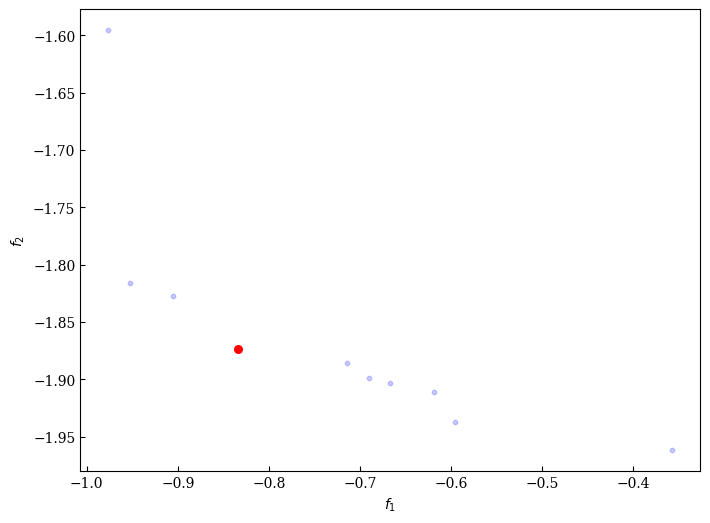
\includegraphics{TargetOptimization_files/figure-pdf/fig-pymoo-parks-output-1.png}

}

\subcaption{\label{fig-pymoo-parks-1}Multi-objective optimization Pareto
front. The selected solution is indicated in red.}

\end{minipage}%
%
\begin{minipage}{0.50\linewidth}

\centering{

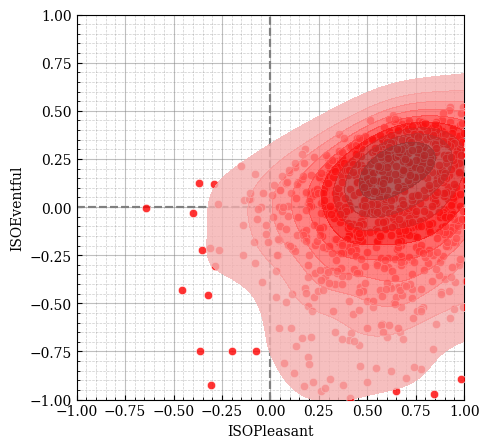
\includegraphics{TargetOptimization_files/figure-pdf/fig-pymoo-parks-output-2.png}

}

\subcaption{\label{fig-pymoo-parks-2}SCM distribution of the derived
target distribution.}

\end{minipage}%

\caption{\label{fig-pymoo-parks}NSGA-II optimization to learn the MSN
parameters which produce the Park ranking.}

\end{figure}%


  \bibliography{../../../../FellowshipRefs.bib,../../FellowshipRefs.bib}



\end{document}
